\documentclass[tikz,border=8pt]{standalone}
\usetikzlibrary{shadings}
\definecolor{bg}{HTML}{FFF6EA}
\definecolor{fur}{HTML}{D9A066}
\definecolor{furdark}{HTML}{B57D45}
\definecolor{furlight}{HTML}{EBC08C}
\definecolor{muzzle}{HTML}{F6E2C4}
\definecolor{pad}{HTML}{F1C9A2}
\definecolor{nose}{HTML}{5A3A2A}
\definecolor{cheek}{HTML}{F2A48F}
\definecolor{patch}{HTML}{F7D08A}
\definecolor{stitch}{HTML}{A56A3C}
\definecolor{ribbon}{HTML}{E8735C}
\begin{document}
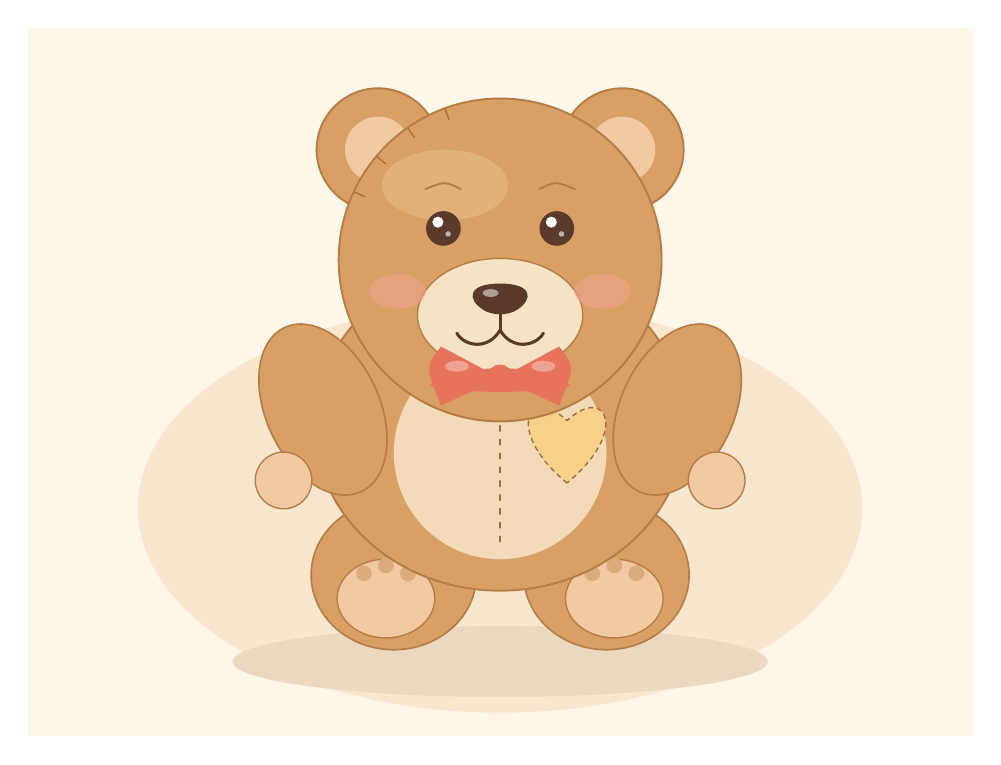
\begin{tikzpicture}[x=1cm,y=1cm,line join=round,line cap=round]
  % canvas 12 x 9 (1200x900 相当)
  \fill[bg] (-6,-4.5) rectangle (6,4.5);
  \fill[furlight!30!bg] (0,-1.6) ellipse (4.6 and 2.6);
  % floor shadow
  \fill[furdark!25!bg] (0,-3.55) ellipse (3.4 and 0.45);

  % ---- legs (behind body, short and round) ----
  \foreach \s in {-1,1}{
    \fill[fur,draw=furdark,line width=0.6pt] (\s*1.35,-2.45) ellipse (1.05 and 0.95);
    % foot pads
    \fill[pad,draw=furdark,line width=0.5pt] (\s*1.45,-2.75) ellipse (0.62 and 0.5);
    \foreach \dx/\dy in {-0.28/0.32,0/0.42,0.28/0.32}{
      \fill[pad!60!furdark] (\s*1.45+\dx,-2.75+\dy) circle (0.1);
    }
  }

  % ---- body (wide, stuffed) ----
  \fill[fur,draw=furdark,line width=0.7pt]
    (0,-0.55) ellipse (2.35 and 2.1);
  % soft belly highlight
  \fill[muzzle,opacity=0.9] (0,-0.9) ellipse (1.35 and 1.35);
  % stitched seam down the belly
  \draw[stitch,line width=0.5pt,dash pattern=on 2pt off 3pt] (0,0.15) -- (0,-2.05);

  % chest patch (heart-shaped appliqué)
  \begin{scope}[shift={(0.85,-0.85)},scale=0.36]
    \fill[patch,draw=stitch,line width=0.5pt,dash pattern=on 1.6pt off 1.6pt]
      (0,-1.2) .. controls (-2.2,0.6) and (-1.4,2.3) .. (0,1.0)
               .. controls (1.4,2.3) and (2.2,0.6) .. (0,-1.2) -- cycle;
  \end{scope}

  % ---- arms (short, round, slightly forward) ----
  \foreach \s in {-1,1}{
    \fill[fur,draw=furdark,line width=0.6pt,rotate around={\s*-25:(\s*2.25,-0.35)}]
      (\s*2.25,-0.35) ellipse (0.72 and 1.15);
    \fill[pad,draw=furdark,line width=0.5pt] (\s*2.75,-1.25) circle (0.36);
  }

  % ---- ears (large, symmetric) ----
  \foreach \s in {-1,1}{
    \fill[fur,draw=furdark,line width=0.7pt] (\s*1.55,2.95) circle (0.78);
    \fill[pad] (\s*1.55,2.95) circle (0.42);
  }

  % ---- head (round) ----
  \fill[fur,draw=furdark,line width=0.7pt] (0,1.55) circle (2.05);
  % head sheen
  \fill[furlight,opacity=0.55] (-0.7,2.5) ellipse (0.8 and 0.45);

  % muzzle
  \fill[muzzle,draw=furdark,line width=0.5pt] (0,0.85) ellipse (1.05 and 0.72);
  % nose (rounded triangle, stitched look)
  \fill[nose] (0,1.25) .. controls (0.42,1.25) and (0.42,1.05) .. (0.22,0.92)
               .. controls (0.1,0.84) and (-0.1,0.84) .. (-0.22,0.92)
               .. controls (-0.42,1.05) and (-0.42,1.25) .. (0,1.25) -- cycle;
  \fill[white,opacity=0.5] (-0.12,1.13) ellipse (0.1 and 0.05);
  % mouth
  \draw[nose,line width=1.1pt] (0,0.92) -- (0,0.66);
  \draw[nose,line width=1.1pt] (0,0.66) .. controls (-0.15,0.4) and (-0.45,0.45) .. (-0.55,0.62);
  \draw[nose,line width=1.1pt] (0,0.66) .. controls (0.15,0.4) and (0.45,0.45) .. (0.55,0.62);

  % eyes (glossy buttons)
  \foreach \s in {-1,1}{
    \fill[nose] (\s*0.72,1.95) circle (0.22);
    \fill[white] (\s*0.72-0.07,2.03) circle (0.07);
    \fill[white,opacity=0.6] (\s*0.72+0.06,1.88) circle (0.035);
  }
  % cheeks
  \foreach \s in {-1,1}{
    \fill[cheek,opacity=0.55] (\s*1.3,1.15) ellipse (0.36 and 0.22);
  }
  % eyebrows (soft)
  \foreach \s in {-1,1}{
    \draw[furdark,line width=0.7pt] (\s*0.5,2.45) .. controls (\s*0.7,2.55) .. (\s*0.95,2.45);
  }

  % ---- neck ribbon ----
  \fill[ribbon] (-0.9,-0.05) .. controls (-0.5,0.25) and (0.5,0.25) .. (0.9,-0.05)
                .. controls (0.5,-0.15) and (-0.5,-0.15) .. (-0.9,-0.05) -- cycle;
  \fill[ribbon] (0,0.05) circle (0.17);
  \fill[ribbon] (0,0.05) -- (-0.75,0.45) .. controls (-0.95,0.2) .. (-0.75,-0.3) -- cycle;
  \fill[ribbon] (0,0.05) -- (0.75,0.45) .. controls (0.95,0.2) .. (0.75,-0.3) -- cycle;
  \fill[white,opacity=0.35] (-0.55,0.2) ellipse (0.15 and 0.07);
  \fill[white,opacity=0.35] (0.55,0.2) ellipse (0.15 and 0.07);

  % stitch marks on the head seam
  \foreach \a in {110,125,140,155}{
    \draw[stitch,line width=0.45pt] (\a:1.9) ++(0,1.55) -- +(\a:0.14);
  }
\end{tikzpicture}
\end{document}
